% =======================================================
% 6. FUNZIONALITÀ DI INTELLIGENZA ARTIFICIALE
% =======================================================
\subsection{Strumenti di Intelligenza Artificiale}
\label{sec:strumenti-ai}
La quinta ed ultima parte è denominata Assistente AI con un singolo bottone dallo stesso nome. 
Quando cliccato appariranno 5 bottoni:
\begin{enumerate}
    \item Riassumi,
    \item Traduci,
    \item Riscrivi,
    \item Distant Writing\textsubscript{G},
    \item Sei Cappelli per Pensare\textsubscript{G}.
\end{enumerate}
I primi tre, così come "Sei Cappelli per Pensare", richiedono di selezionare preventivamente un blocco di testo: se si clicca uno di questi 
bottoni senza aver selezionato nulla, il sistema mostra un messaggio di avviso temporaneo (\emph{Seleziona del testo prima di richiedere 
questa operazione}, oppure \emph{Seleziona del testo da tradurre prima di continuare} nel caso della traduzione\textsubscript{G}) e la richiesta non viene 
inviata. Una volta selezionato del testo valido, l'operazione interrogherà l'LLM\textsubscript{G} con la richiesta scelta, e apparirà una nuova finestra 
di attesa per la risposta dell'elaborazione da parte dell'LLM.
\textbf{Distant Writing è l'unica eccezione}: non richiede alcuna selezione di testo, in quanto genera contenuto nuovo a partire da un 
prompt\textsubscript{G} inserito dall'utente (vedi Sezione~\ref{sec:distant-writing}).
La traduzione inoltre permette la scelta della lingua in cui tradurre il testo tra inglese, francese, spagnolo e tedesco.

\begin{figure}[H]
    \centering
    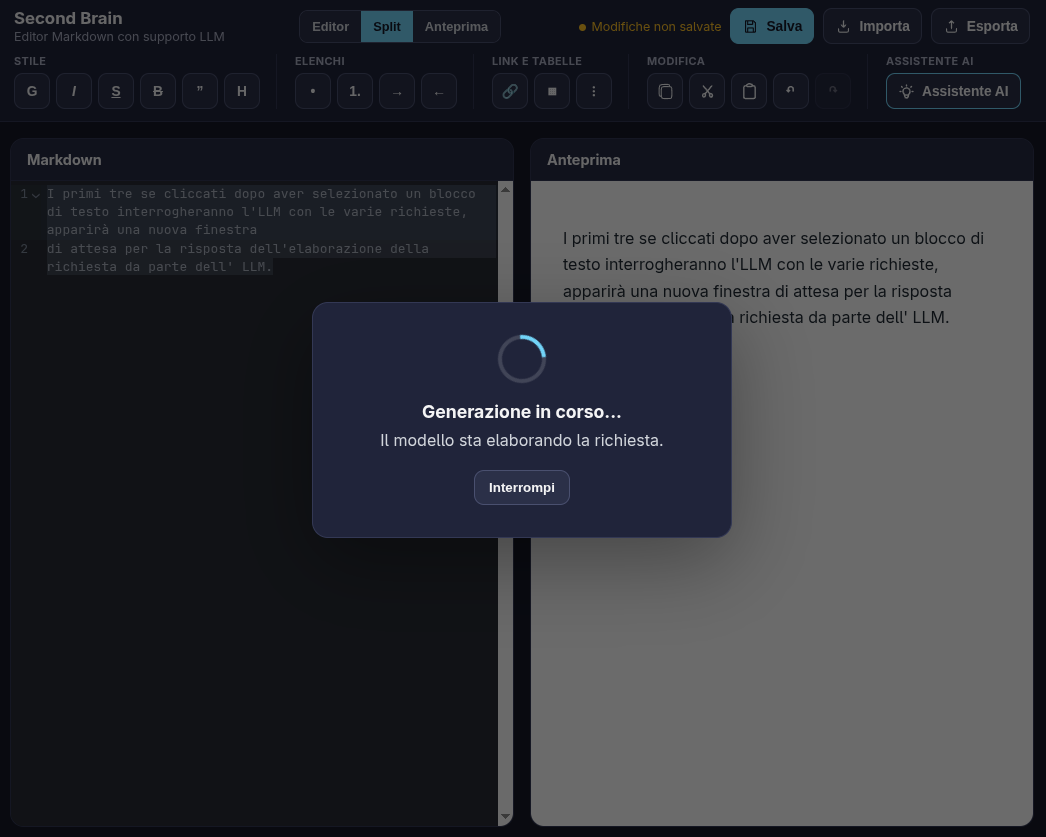
\includegraphics[width=0.6\textwidth]{img/elaborazione.png}
    \caption{Finestra durante l'elaborazione della richiesta all'LLM}
 \end{figure}

 Se la richiesta va a buon fine si presenterà un'altra finestra con la proposta dell'LLM la quale può essere rifiutata, rigenerata o accettata.
 Se accettata essa verrà inserita nell'editor, se rigenerata verrà fatta una nuova richiesta all'LLM mentre se rifiutata si chiuderà semplicemente 
 la finestra senza alcuna modifica al file.

 \begin{figure}[H]
    \centering
    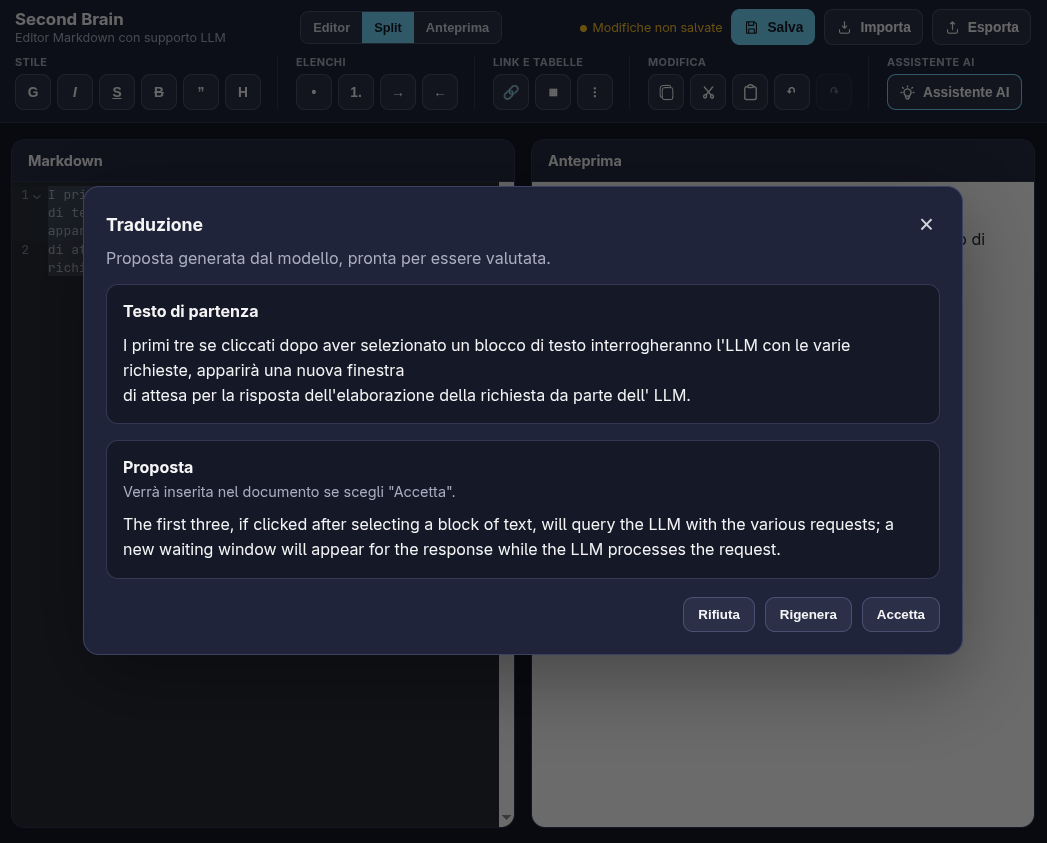
\includegraphics[width=0.6\textwidth]{img/proposta.png}
    \caption{Finestra di proposta dell'LLM}
 \end{figure}

\subsubsection{Distant Writing}
\label{sec:distant-writing}
Il distant Writing è una funzionalità che permette la generazione di testo da parte dell'LLM tramite un prompt inserito dall'utente.

 \begin{figure}[H]
    \centering
    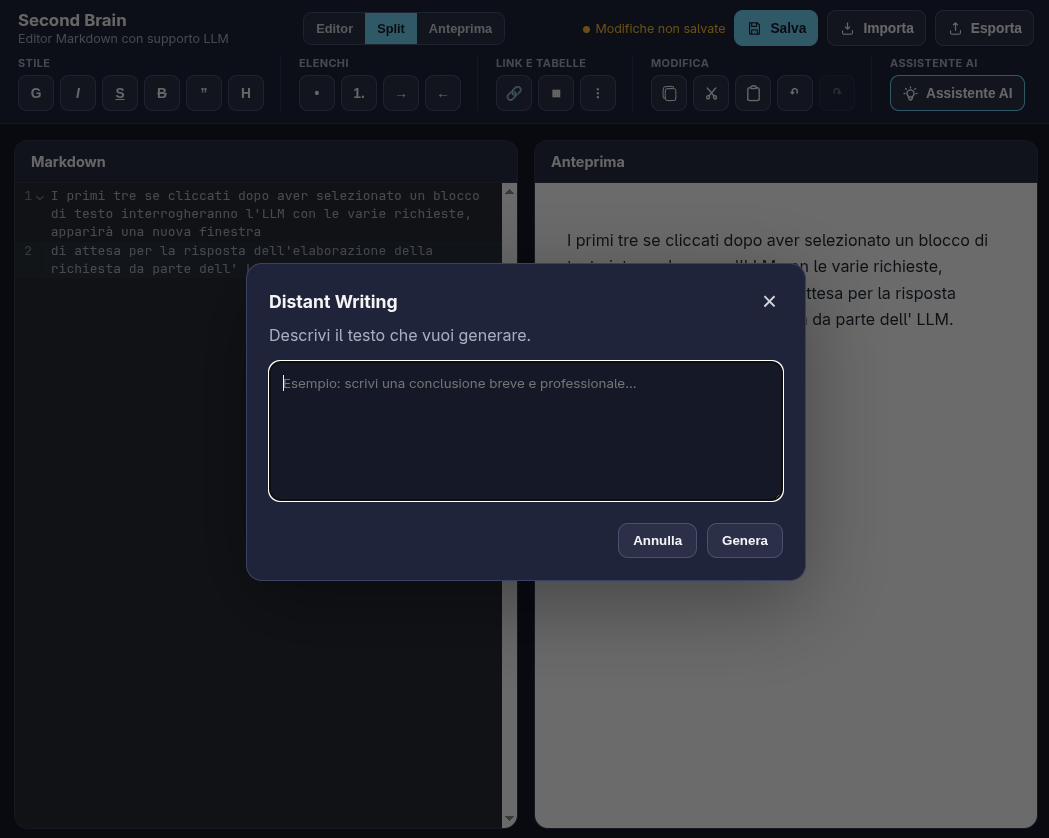
\includegraphics[width=0.6\textwidth]{img/distant_writing.png}
    \caption{Finestra di richiesta di Distant Writing}
 \end{figure}

\subsubsection{Analisi Critica: I "Sei Cappelli di De Bono"}
L'ultimo bottone ovvero "Sei cappelli per pensare" se cliccato ne presenta altri che sono:
\begin{itemize}
    \item Bianco - fatti e dati,
    \item Rosso - emozioni,
    \item Nero - criticità
    \item Giallo - benefici,
    \item Verde - creatività,
    \item Blu - visione d'insieme.
\end{itemize}
Essi si basano sui "Sei cappelli per pensare" di Edward de Bono. 
Dopo aver selezionato del testo, quando clicco un cappello viene fatta una richiesta all'LLM di interpretare il testo selezionato 
dal punto di vista del cappello selezionato.